\subsection{Graph}
\begin{defi}
	Ein Graph $G$ ist ein geordnetes Paar $(V,W)$, wobei $V$ eine Menge von Knoten und $E$ eine Menge von Kanten bezeichnet. Dabei sind Kanten paarweise Verbindungen zwischen Knoten. Diese Kanten können mit sog. Gewichten versehen werden. Grundsätzlich unterscheidet man \emph{gerichtete} und \emph{ungerichtete} Kanten. Sind alle Paare $(v_1, v_2) \in E$ gerichtet, d. h. $(v_1, v_2) \neq (v_2, v_1)$, dann spricht man von einem gerichteten Graphen (\emph{Digraph}). Ein ungerichteter Graph, bei dem jeder Knoten mit allen anderen Knoten verbunden ist, heißt \emph{vollständig}.
\end{defi}

\begin{bsp}
	Abbildung \ref{digraph} zeigt ein Beispiel für einen Digraphen mit $V=\{1,2,3,4,5,6\}$ und den Kanten
	\begin{gather*}
		E=\{(1,4), (2,1), (2,3), (3,6), (4,2), (4,3), (4,5), (5,1), (5,3), (5,6), (6,4)\}.
	\end{gather*}
	\label{bsp:digraph}
\end{bsp}

\begin{figure}[!h]
	\centering
	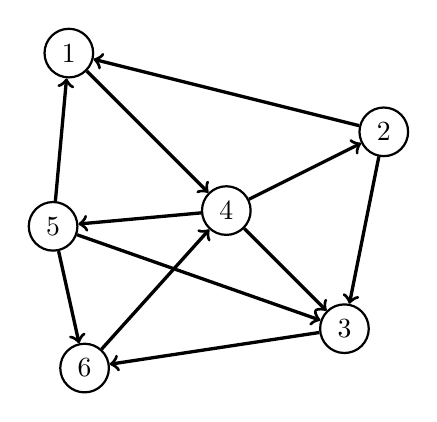
\begin{tikzpicture}
		\begin{scope}[every node/.style={circle,thick,draw}]
			\node (A) at (0,0) {1};
			\node (B) at (4,-1) {2};
			\node (C) at (3.5,-3.5) {3};
			\node (D) at (2,-2) {4};
			\node (E) at (-0.2,-2.2) {5};
			\node (F) at (0.2,-4) {6};
		\end{scope}

		\begin{scope}[every edge/.style={draw=black, very thick}]
			\path [->] (A) edge (D);
			\path [->] (B) edge (A);
			\path [->] (B) edge (C);
			\path [->] (C) edge (F);
			\path [->] (D) edge (B);
			\path [->] (D) edge (E);
			\path [->] (D) edge (C);
			\path [->] (E) edge (A);
			\path [->] (E) edge (F);
			\path [->] (E) edge (C);
			\path [->] (F) edge (D);
		\end{scope}
	\end{tikzpicture}
	\caption{Beispiel für einen Digraphen}
	\label{digraph}
\end{figure}

\begin{proposition}
	Sei $G=(E, V)$ ein Graph. Dann gilt:
	\begin{enumerate}[label=(\roman*)]
		\item Für die Anzahl von Kanten in einem Digraphen ohne Schleifen und Mehrfachkanten gilt
		      \begin{gather*}
			      |E| \le |V|(|V| - 1).
		      \end{gather*}

		\item Für die Anzahl von Kanten in einem ungerichteten Graphen ohne Schleifen und Mehrfachkanten gilt
		      \begin{gather*}
			      |E| \le \frac{1}{2} |V|(|V| - 1).
		      \end{gather*}
	\end{enumerate}
	In vollständigen Graphen gilt jeweils Gleichheit.
\end{proposition}

\begin{proof}[Beweis (nur für $(i)$ )]
	Jeder Knoten hat höchstens alle Knoten außer sich selbst als Nachbar, er hat also $|V| - 1$ Nachbarn. Da dies für jeden Knoten des Graphen möglich ist folgt die Behauptung.
\end{proof}

Eine weitere Möglichkeit Graphen anzugeben sind sog. \emph{Adjazenzlisten} oder \emph{Adjazenzmatrizen}. Hierbei listet man für die jeweiligen Knoten alle Nachbarn auf (Adjazenzliste) bzw. setzt in einer Matrix den Eintrag $a_{ij}$ auf $1$, falls es eine Kante vom Knoten $v_1$ nach $v_2$ gibt, bzw. allgemein:
\begin{defi}[Adjazenzmatrix]
	Eine Adjazenzmatrix eines Graphen $G=(V,E)$ ist eine $|V| \times |V|$-Matrix $A = (a_{ij})$ mit
	\begin{gather*}
		a_{ij} = \begin{cases}
			1 & \text{falls } (i,j) \in E \\
			0 & \text{sonst.}
		\end{cases}
	\end{gather*}
\end{defi}

\begin{anm}
	Offensichtlich sind Adjazenzmatrizen von ungerichteten Graphen symmetrisch.
\end{anm}

Für den im Beispiel \ref{bsp:digraph} definierten Graph sieht die Adjazenzmatrix folgendermaßen aus:
\begin{gather*}
	\bordermatrix{
		& 1 & 2 & 3 & 4 & 5 & 6 \cr
		1 & 0 & 0 & 0 & 1 & 0 & 0 \cr
		2 & 1 & 0 & 1 & 0 & 0 & 0 \cr
		3 & 0 & 0 & 0 & 0 & 0 & 1 \cr
		4 & 0 & 1 & 1 & 0 & 1 & 0 \cr
		5 & 1 & 0 & 1 & 0 & 0 & 1 \cr
		6 & 0 & 0 & 0 & 1 & 0 & 0 \cr
	}
\end{gather*}

Für gewichtete Graphen eignet sich die Darstellung in Form von Adjazenzmatrizen auch: hierbei kann anstatt des Wertes $1$ in der Adjazenzmatrix einfach das Gewicht der jeweiligen Kante eingetragen werden.

Für gerichtete Graphen wollen wir nun weitere Begriffe einführen:

\begin{defi}
	Sei $G=(V,E)$ ein gerichteter Graph. Dann definieren wir
	\begin{itemize}
		\item die eingehende Nachbarmenge von $v \in V$:
		\begin{gather*}
			N^{+}(v) = \{u \in V \mid (u,v) \in E \}
		\end{gather*}

		\item die ausgehende Nachbarmenge von $v \in V$:
		\begin{gather*}
			N^{-}(v) = \{w \in V \mid (v,w) \in E \}
		\end{gather*}

		\item den Eingangsgrad von $v \in V$:
		\begin{gather*}
			deg_{in}(v) = \big| N^{+}(v) \big|
		\end{gather*}

		\item den Ausgangsgrad von $v \in V$:
		\begin{gather*}
			deg_{out}(v) = \big| N^{-}(v) \big|
		\end{gather*}
	\end{itemize}
\end{defi}

Setzt man Graphen als Datenstruktur ein, so ist es häufig das Ziel, den (kürzesten) Weg zwischen zwei Knoten zu finden. Dies führt uns zur nächsten

\begin{defi}[Pfade]
	Es sei $G=(V,E)$ ein Graph. Ein Pfad ist eine Folge von paarweise verschiedenen Knoten $u_1, \dots, u_k \in V$, wobei $(u_i, u_{i+1}) \in E$ für alle $i \in \{1, \dots, k-1\}$. \\

	Die Länge eines Pfades ist die Anzahl der Kanten (falls die Kanten von $G$ nicht gewichtet sind) bzw. die Summe der Kantengewichte. Dabei sei $d(u,v)$ die Länge des kürzesten Pfades von $u$ nach $v$. Der Durchmesser $D$ sei definiert durch $D = \underset{u,v \in V}{\max}{d(u,v)}$. \\

	Ist $v_1 = v_k$, so heißt der Pfad $(v_1, \dots, v_k)$ Zyklus \footnote{Hierbei wird allerding i. d. R. nicht verlangt, dass $(v_1, \dots, v_k)$ ein Pfad ist -- es genügt dass $(v_1, \dots, v_k)$ ein Weg ist (die Knoten müssen also nicht paarweise verschieden sein).}. Gilt zusätzlich $v_i \neq v_j$ für $i,j \in \{1, \dots, k-1\}$ mit $i \neq j$, dann heißt der Pfad Kreis.
\end{defi}

\begin{defi}
	Es sei $G = (V,E)$ ein Graph mit $|V| \ge 1$. $G$ heißt \emph{zusammenhängend}, falls für jedes Knotenpaar $(u,v)$ mit $u,v \in E$ ein Weg von $u$ nach $v$ in $G$ exisitert.
\end{defi}

\subsubsection{Breitensuche (Breadth-First-Search)}
Bei der Breitensuche handelt es sich um ein Verfahren zum Durchsuchen (oder nur Durchlaufen) der Knoten eines Graphen. Hierbei werden zunächst alle Knoten beschritten, die vom Ausgangsknoten direkt erreichbar sind. Erst danach werden Folgeknoten beschritten. Dazu verwendet man in der Regel eine Warteschlange (vgl. Abschnitt \emph{Queue}). \\ \\
Informell lässt sich die Breitensuche folgendermaßen beschreiben:
\begin{enumerate}
	\item Bestimme den Knoten, an dem die Suche beginnen soll, markiere ihn als besucht und füge ihn der Warteschlange hinzu
	\item Entnimm einen Knoten vom Beginn der Warteschlange
	\begin{itemize}
		\item Falls der entnommene Knoten der gesuchte Knoten ist, brich die Suche ab (und gebe den Knoten oder ``gefunden'' zurück)
		\item Andernfalls hänge alle unmarkierten Nachfolge diese Knoten ans Ende der Warteschlange an und markiere sie als besucht
	\end{itemize}
	\item Prüfe ob die Warteschlange leer ist. Falls ja, beende die Suche (gesuchtes Element wurde nicht gefunden)
	\item Wiederhole Schritt 2.
\end{enumerate}
Als Pseudocode könnte die Breitensuche folgendermaßen aussehen:
\begin{algorithm}[H]
	\caption{Breitensuche mit Startknoten $start$ und gesuchtem Knoten $goal$}
	 \begin{algorithmic}
		 \Procedure{bfs}{$start, goal$}
				\For{\textbf{all node} $i$} \Comment{Anfangs sind keine Knoten besucht}
					\State{$visited[i] \gets false$}
				\EndFor
				\State{$queue.$\Call{push}{$start$}}
				\State{$visited[start] \gets true$}

				\While{\textbf{not} $queue.$\Call{empty}{}}
					\State{$node \gets queue.$\Call{pop}{}}
					\If{$node$ \textbf{is} $goal$}
						\State{\Return{$true$}}
					\EndIf
					\For{$child$ \textbf{in} $neighbors[node]$}
						\If{\textbf{not} $visited[child]$}
							\State{$queue.$\Call{push}{$child$}}
							\State{$visited[child] \gets true$}
						\EndIf
					\EndFor
				\EndWhile
				\State{\Return{$false$}}
		 \EndProcedure
	 \end{algorithmic}
\end{algorithm}

\begin{proposition}[Laufzeit]
	Im schlechtesten Fall müssen alle möglichen Pfade zu allen möglichen Knoten betrachtet werden, daher gilt für die Laufzeit der Breitensuche
	\begin{itemize}
		\item Falls Adjazenzlisten benutzt werden: $\mathcal{O}(|V| + |E|)$
		\item Falls Adjazenzmatrizen benutzt werden: $\mathcal{O}(|V|^2)$.
	\end{itemize}
\end{proposition}

\begin{bsp}
	Interpretiert man einen Graphen als Baum und definiert die Reihenfolge der Nachfolger eines Knotens von links nach rechts, so würde man den Baum in Abbildung \ref{bfstree} Ebene für Ebene und innerhalb der Ebenen von links nach rechts durchlaufen und erhielte dann die Reihenfolge
	\begin{gather*}
		17 \rightarrow 4 \rightarrow 11 \rightarrow 18 \rightarrow 3 \rightarrow 9 \rightarrow 13 .
	\end{gather*}
\end{bsp}

\begin{figure}[!h]
	\centering
	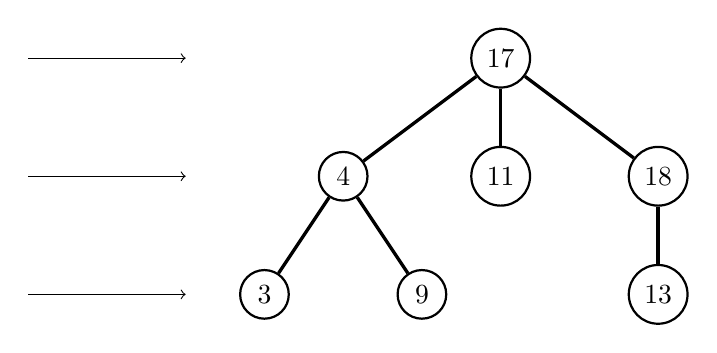
\begin{tikzpicture}
		\begin{scope}[every node/.style={circle,thick,draw}]
			\node (A) at (0,0) {17};
			\node (B) at (-2,-1.5) {4};
			\node (C) at (0,-1.5) {11};
			\node (D) at (2, -1.5) {18};
			\node (E) at (-3, -3) {3};
			\node (F) at (-1, -3) {9};
			\node (G) at (2, -3) {13};
		\end{scope}

		\begin{scope}[every edge/.style={draw=black, very thick}]
			\path [-] (A) edge (B);
			\path [-] (A) edge (C);
			\path [-] (A) edge (D);
			\path [-] (B) edge (E);
			\path [-] (B) edge (F);
			\path [-] (D) edge (G);
		\end{scope}

		\draw [->] (-6,0) -- (-4,0);
		\draw [->] (-6,-1.5) -- (-4,-1.5);
		\draw [->] (-6,-3) -- (-4,-3);


	\end{tikzpicture}
	\caption{Breitensuche in einem Baum}
	\label{bfstree}
\end{figure}
\subsubsection{Tiefensuche (Depth-First-Search)}
Wie auch die Breitensuche ist die \emph{Tiefensuche} ein Verfahren zum Suchen von Knoten in einem Graphen. Im Gegensatz zur Breitensuche wird ein Pfad zunächst vollständig in die Tiefe beschritten, bevor abzweigende Pfade beschritten werden.\\
Informell lässt sich die Tiefensuche folgendermaßen beschreiben:
\begin{enumerate}
	\item Bestimme den Startknoten
	\item Bestimme alle Nachfolger bzw. Nachbarn des Knotens und speichere alle noch nicht erschlossenen Nachfolger in einem Stack
	\item Rufe rekursiv für jeden Knotne in dem Stack die Tiefensuche auf
	\begin{itemize}
		\item Falls das gesuchte Element gefunden wurde breche ab
		\item Falls es keine nicht erschlossenen Nachfolger mehr gibt, lösche den obersten Knoten aus dem Stack und rufe für den jetzt oberen Knoten im Stack die Tiefensuche auf
	\end{itemize}
\end{enumerate}

In Pseudocode könnte die Tiefensuche folgendermaßen aussehen:
\begin{algorithm}[H]
	\caption{Tiefensuche mit Startknoten $start$ und gesuchtem Knoten $goal$}
	\begin{algorithmic}
		\Procedure{dfs}{$start, goal$}
			\If{$start$ \textbf{is} $goal$}
				\State{\Return $start$}
			\EndIf
			\State{$stack \gets$ \Call{neighbors}{$start$}}
			\While{$stack$ \textbf{is not empty}}
				\State{$node \gets$ \Call{pop}{$stack$}}
				\State{\Call{dfs}{$node, goal$}}
			\EndWhile
		\EndProcedure
	\end{algorithmic}
\end{algorithm}

\begin{bsp}
	Mit dem selben Baum wie in Abbildung \ref{bfstree} erhält man nun mit der Tiefensuche (siehe Abb. \ref{dfstree}) die Reihenfolge
	\begin{gather*}
		17 \rightarrow 4 \rightarrow 3 \rightarrow 9 \rightarrow 11 \rightarrow 18 \rightarrow 13 
	\end{gather*}
\end{bsp}

\begin{figure}[!h]
	\centering
	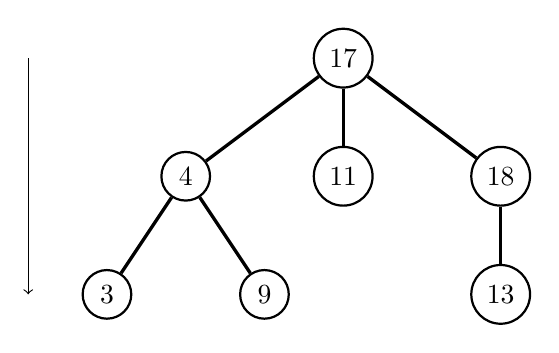
\begin{tikzpicture}
		\begin{scope}[every node/.style={circle,thick,draw}]
			\node (A) at (0,0) {17};
			\node (B) at (-2,-1.5) {4};
			\node (C) at (0,-1.5) {11};
			\node (D) at (2, -1.5) {18};
			\node (E) at (-3, -3) {3};
			\node (F) at (-1, -3) {9};
			\node (G) at (2, -3) {13};
		\end{scope}

		\begin{scope}[every edge/.style={draw=black, very thick}]
			\path [-] (A) edge (B);
			\path [-] (A) edge (C);
			\path [-] (A) edge (D);
			\path [-] (B) edge (E);
			\path [-] (B) edge (F);
			\path [-] (D) edge (G);
		\end{scope}

		\draw [->] (-4,0) -- (-4,-3);


	\end{tikzpicture}
	\caption{Tiefensuche in einem Baum}
	\label{dfstree}
\end{figure}